\documentclass[]{auvsi_doc}
\setkeys{auvsi_doc.cls}{
	AUVSITitle={Path Planner Testing Procedures and Results},
	AUVSILogoPath={./../logo.pdf}
}

\usepackage{hyperref}
\hypersetup{
	colorlinks=true,
	linkcolor=blue,
	filecolor=magenta,
	urlcolor=cyan,
}

\urlstyle{same}

\begin{document}

\begin{AUVSITitlePage}
\begin{artifacttable}
\entry{CT-003, 0.1, 02-21-2019, Initial conception, John Akagi, Andrew Torgesen}
\entry{CT-003, 0.1, 04-4-2019, Addition of Hardware Testing, John Akagi, Andrew Torgesen}
% additional \entry{} commands for extra rows in the revision table, if needed
\end{artifacttable}
\end{AUVSITitlePage}

\section*{Purpose}

The purpose of this artifact is to explain the test procedures used to verify that the path planner is working correctly in both simulation and hardware.

\section*{Procedure}

In order to test the path planner, 5 simulations were run. Each simulation had 10 obstacles and 5 waypoints, each of which were chosen randomly.
The locations of the obstacles and waypoints were written to a file and then the path planner planned a path, starting from the origin, that attempted to fly through each waypoint and avoid each obstacle.
Once the path was planned, the simulated drone would fly the path and the position data was continually written to a file. Once the simulation finished, the distances between the waypoints and vehicle and obstacle and vehicle are computed.
These distances are used to determine if the vehicle was close enough to the waypoint and if the vehicle hit the obstacle.
These values were then compared with the key success measures. For reference, an excellent rating is defined in the key success measures as no more than 1 obstacle hit (10\%) and flying within 20 feet (6 m) of each waypoint.

For hardware testing, three waypoints are chosen that are safe to fly through. These waypoints should be picked to be at an altitude of at least 10 m and should not be over buildings or people. The waypoints are found using GPS coordinates and then changed to North East Down (NED) coordinates centered on the reference launch location. The path is planned while the aircraft is being flow via remote control until an acceptable path is found. Once a suitable path is found, the plane is transferred to autopilot and immediately attempts to fly the planned path.

\section*{Results}

The results of the 5 simulations can be seen in Table \ref{tab:results}. In the five simulations, the vehicle only hit a single obstacle and was able to get within 5 meters on all but one waypoint.
These results place the vehicle in the excellent category as defined by the key success measures.

While testing hardware, there was a strong wind so the plane had difficulty staying directly on the planned path. However, it was able to follow the path and hit the waypoints despite this. As a result of the wind, the plane was not as accurate as when tested in simulation, but we were still able to get within 15 ft of each waypoint. The flight is shown in Figure \ref{fig:flight} where the waypoints are the yellow points, the planned path is in green, and the actual flown path is in white.

\begin{table}[h!]

\caption{Table of results showing the number of obstacles hit and the minimum distance between the UAV and each waypoint.}
\label{tab:results}
\begin{tabular} {|l|l|l|l|l|l|l|}
\hline
Test No. & Waypoint 1&Waypoint 2&Waypoint 3&Waypoint 4&Waypoint 5& Obstacles Hit\\
\hline
1 & .750 m& .128 m& .092 m& .430 m& .688 m & 0\\
2 & 1.058 m &.127 m & .180 m & .376 m & .328m & 0\\
3& .602 m& .625 m&.158 m& .204 m& .122 m& 0\\
4& .427 m & .351 m & .042 m & .018 m& 69.7m& 1\\
5& .152 m& .085 m& .011 m & 1.11 m & .90 m& 0\\
\hline
\end{tabular}
\end{table}

\begin{figure}
    \centering
    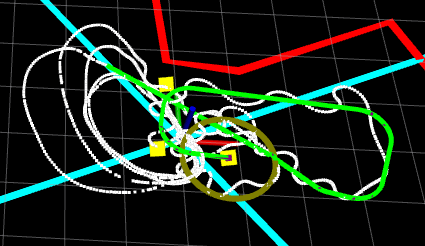
\includegraphics[width=.75\textwidth]{WaypointTest.png}
    \caption{The flight path is shown for the hardware test. The yellow points mark the desired waypoints, the green line shows the desired path, and the white line shows the actual flown path. The golden circle shows the final loiter location for the plane to fly once the planned path is flown. As a result of strong winds, the plane had difficulty staying perfectly on the planned path but was still able to follow the path and hit the waypoints.}
    \label{fig:flight}
\end{figure}


\section*{Conclusion}

Overall, the path planning and path following algorithms work well. The vehicle was able to achieve an excellent rating, as defined by the key success measures.
However, some work is still needed to determine why the plane had difficulty hitting the last waypoint on the 4th trial. However, since the simulations can be run repeatedly multiple times, this should be easy to determine.
Although it is likely that performance will be degraded when the algorithms are running on the actual plane since more variables, unknowns, and disturbances will be present, the algorithms have been proven to work to the level desired.

% document contents (see below for LaTex commands that make your life easier)

\end{document}
